\begin{frame}{Human-Human Authentication}

\begin{itemize}
\item User authentication 
\begin{itemize}
\item Differentiate one human user from another
\end{itemize}
\item Prominent authentication approaches
\begin{itemize}
\item Passwords
\item Traditional biometrics
\end{itemize}
\end{itemize}
\end{frame}



\begin{frame}{Limitations of Existing User Authentication Solutions}

\begin{itemize}
\item Passwords 
\begin{itemize}
\item Either insecure or unusable 
\end{itemize}
\item Traditional biometrics (e.g., fingerprints)
\begin{itemize}
\item Invasive
\item High rejection rates
\item Require additional hardware
\item Susceptible to impersonation or spoofing 
\end{itemize}
\end{itemize}

\begin{overlayarea}{\textwidth}{0.45\textheight}
\only<2>{
\begin{center}
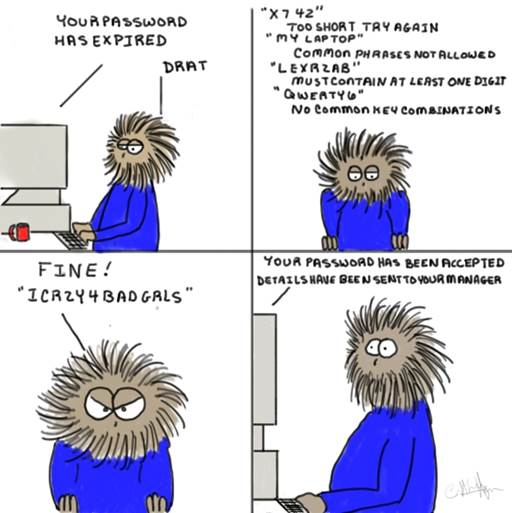
\includegraphics[width=0.3\linewidth]{Figures/password_usability}
\end{center}
}

\only<3>{
\begin{center}
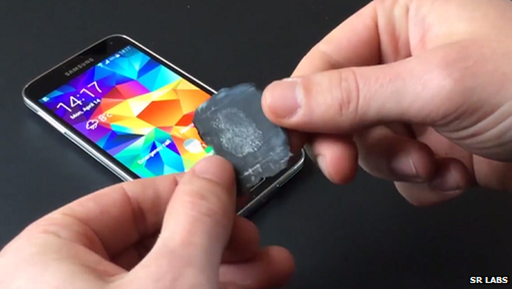
\includegraphics[width=0.3\linewidth]{Figures/spoofing}
\end{center}
}
\end{overlayarea}

\end{frame}



\begin{frame}{Behavioral biometrics}




\begin{itemize}
\item Keystroke dynamics \hfill {\footnotesize{[Monrose et al. ; CCS'97]}}
\item Mouse movement patterns \hfill {\footnotesize{[Zheng et al.; CCS'11]}}
\item Touch gesture biometrics
\begin{itemize}
\item Sliding horizontally and vertically \hfill {\footnotesize{[Frank et al. ; TIFS'13]}}
\item Sliding up, down, left,  and right and tap \hfill {\footnotesize{[Li et al.; NDSS'13]}}
\item Horizontal slide and the pattern unlock  \hfill {\footnotesize{[Luca et al.; CHI'12]}}
\end{itemize}
\end{itemize}


\begin{center}
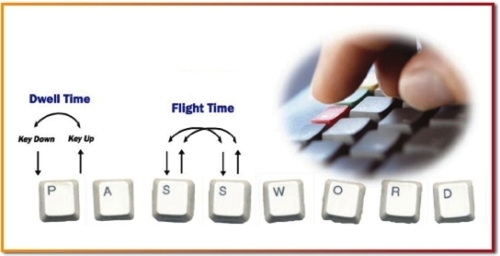
\includegraphics[width=0.3\linewidth]{Figures/bio2}
\end{center}
\end{frame}




\begin{frame}{Gametrics}


\begin{itemize}

\item Interactive game-based behavioral biometrics

\item Why games?

\begin{itemize}
	\item Fully supported by web browsers and touch screen devices
	\item Randomized, interactive and cognitive nature
	\item Sufficient cues can be extracted in a short period of time 
	
\end{itemize}

\end{itemize}

\end{frame}







\begin{frame}{Game Cognitive Task}

\begin{center}
%	\includemedia[
%	activate=pageopen,
%	width=258pt,height=156pt,
%	]{}{Figures/game.swf}
	
	\includemedia[width=0.6\linewidth,height=0.6\linewidth,activate=pageopen,
	passcontext,
	transparent,
	addresource=game.mp4,
	flashvars={source=game.mp4}
	]{
\includegraphics[width=0.6\linewidth]{Figures/game.mp4}}{VPlayer.swf}
	
\end{center}


\end{frame}


\begin{frame}{Features \& Classification Metrics}
\begin{itemize}
\item Features
\begin{itemize}
\item Mouse dynamics / touch gesture  
\item Cognitive ability
\item Others (i.e., distance-based features)
\end{itemize}

\item Classifier
\begin{itemize}
\item Random forest
\end{itemize}

\item Classification metrics 
\begin{itemize}
\item \textbf{False Positive Rate: } Measures the security 
\item \textbf{False Negative Rate:} Measures the usability

\end{itemize}
\end{itemize}

\end{frame}



\begin{frame}{Inter- \& Intra- Session Analysis}
\begin{itemize}
\item Web-based study (MTurk)
\item Data collection methodology:
\begin{itemize}
\item Day 1: 98 participants -- 60 challenges
\item Day 2: 62 participants -- 36 challenges
\item Day 3: 29 participants -- 36 challenges
\end{itemize}

\item Number of successfully completed challenges = 9076
\item Average solving time = 7.5s
\end{itemize}

\end{frame}


\begin{frame}{Inter- \& Intra-Session Results}
%\only<1>{
%\begin{center}
%\includegraphics[width=0.9\linewidth]{Figures/bio-online}
%\end{center}
%}
%
%\only<2>{
%Best results acquired by merging 2 instances and use user specific model
\begin{center}
%\includegraphics[width=0.9\linewidth]{Figures/bio-online-best}
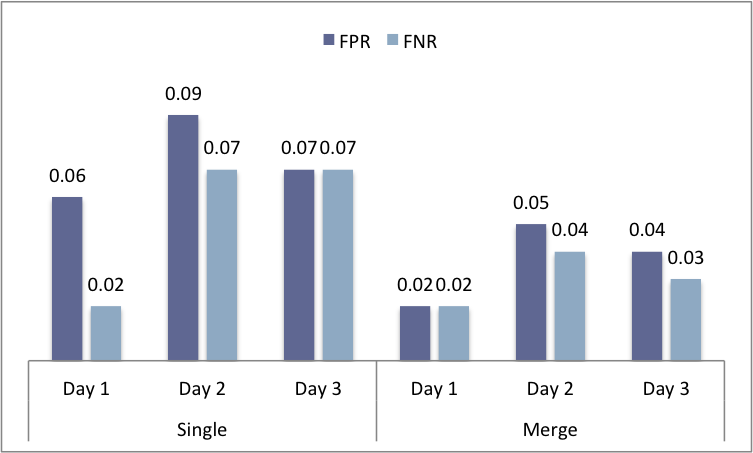
\includegraphics[width=0.9\linewidth]{Figures/result1}
\end{center}
%}

\end{frame}





\begin{frame}{Interactive Biometrics Discussion}

\begin{itemize}
\item Efficiency
\begin{itemize}
\item Short enrollment time
\item Short time to identify the user
\item Building and updating the classifier and testing a new instance take short time
\end{itemize}

\item{Application Scenarios}
\begin{itemize}
\item Point-of-entry
\item Integrated with graphical passwords
\item Fall-back authentication
\end{itemize}

\end{itemize}

\end{frame}


\begin{frame}{Interactive Biometrics Limitations and Future Work}

\begin{itemize}
\item Study the effect of user's behavior variation on the accuracy

\item Test the accuracy when switching devices or hardware

\item  Add more complexity to the game challenges to increase the level of interaction, and improve the overall usability and security

\end{itemize}

\end{frame}